\documentclass[aspectratio=169]{beamer}
\usepackage[utf8]{inputenc}
\usepackage{transparent}
\usepackage{hyperref}
\usepackage{pgf}
\usepackage{dsfont}
\usepackage{algorithm}
\usepackage{algorithmic}
\usepackage{subcaption}
\usepackage{booktabs}

% here comes my custom theme for university of Bamberg

\logo{\pgfputat{\pgfxy(-1.25,4.25)}{\pgfbox[center,base]{\transparent{0.7} 
\includegraphics[width=.15\textwidth]{uni_bamberg.png}}}}


\newcommand{\nologo}{\setbeamertemplate{logo}{}} % command to set the logo to nothing
\newcommand{\biglogo}{\setbeamertemplate{logo}{\pgfputat{\pgfxy(-2,4)}{\pgfbox[center,base]{ 
\includegraphics[width=.24\textwidth]{uni_bamberg.png}}}}} 

% theming and colors and stuff
\usetheme[progressbar=frametitle, block = fill]{metropolis}
\definecolor{uniblau}{RGB}{4, 66, 119} %#044277
\definecolor{niceorange}{RGB}{255, 128, 0} %#ff8000
\definecolor{nicegray}{RGB}{221, 239, 244} %#ddeff4
\setbeamercolor{palette primary}{bg=uniblau, fg=white}
\setbeamercolor{normal text}{fg=uniblau, bg=white}
\setbeamercolor{itemize item}{fg=niceorange}
\setbeamercolor{itemize subitem}{fg=niceorange}
\setbeamercolor{itemize subsubitem}{fg=niceorange}
\setbeamercolor{enumerate item}{fg=niceorange}
\setbeamercolor{enumerate subitem}{fg=niceorange}
\setbeamercolor{enumerate subsubitem}{fg=niceorange}
\setbeamercolor{block body}{bg=nicegray}
\setbeamercolor{block title}{bg=niceorange,fg=white}
\renewcommand\UrlFont{\color{niceorange}\rmfamily}

% own commands for highlighting
\newcommand{\pop}[1]{{\color{niceorange}\textbf{#1}}}

\def\ps@titlepage{\setbeamertemplate{footline}{}}
\makeatletter
\setbeamertemplate{frame footer}{\tiny{xAI-Proj-M - Model Evaluation - Benedikt Marsiske }}

% custom python style

%title page
\title{Model Evaluation  -- The Effect of Noisy Data}
\subtitle{Explainable Machine Learning - Deep Learning Life Cycle}
\author{Jonas Amling \and Baptiste Patrice Francis Bony \and Benedikt Markus Marsiske}
\institute{University of Bamberg}
\date{\today} 

\begin{document}
% titleframe
{\biglogo
	\setbeamertemplate{footline}{} 
	\begin{frame}{}
		\titlepage
	\end{frame}
}

\begin{frame}{Table of contents}
	\tableofcontents
\end{frame}


{\nologo
\section{Research Question}
	\begin{frame}{Research Question and Introduction}
	Focus for evaluating our trained model:
	\begin{itemize}
		\item How well does the model perform?
		\item Is there a difference between the classes?
		\item How robust is our model?
	\end{itemize}
	\pause
	Specific Research Question: \pop{How does the model perform on distorted data? Does the usage of distorted test data lead to a worse model performance compared to the same test data without distortion?} 
	\end{frame}

\section{Basic Model Evaluation}
	\begin{frame}{Model Performance - Training Data}
	How well did our model perform on our training data?
		\begin{figure}
			\centering
			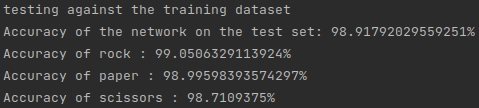
\includegraphics[width=0.8\textwidth]{img/TestAccuracy_final_train.png}
			\caption{Accuracy at the end of training}
		\end{figure}
	\end{frame}

	\begin{frame}{Confusion Matrix - Training Data}
		\begin{columns}
			\begin{column}{.5\textwidth}
				\begin{figure}
					\centering
					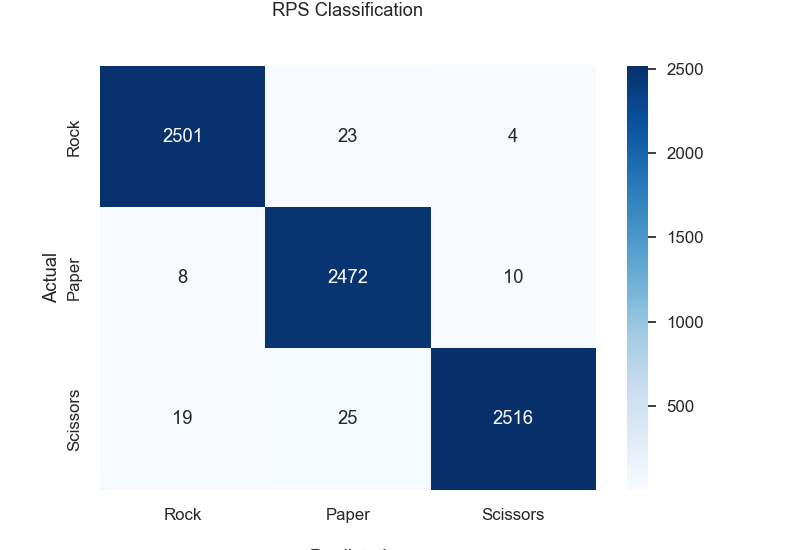
\includegraphics[width=1\textwidth]{img/CFM_final_train_numeric.png}
					\caption{Numeric CM of Training Data}
				\end{figure}      
			\end{column}
			\begin{column}{.5\textwidth}
				\begin{figure}
					\centering
					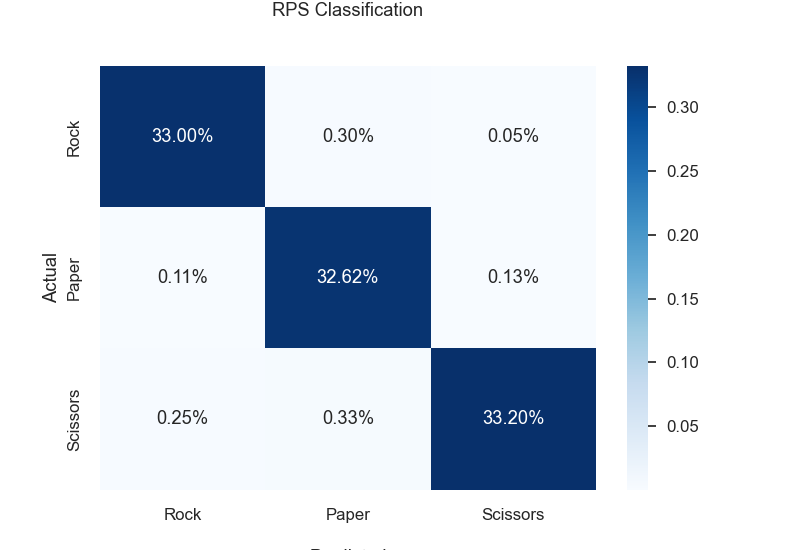
\includegraphics[width=1\textwidth]{img/CFM_final_train_percent.png}
					\caption{CM of Training Data (in \%)}
				\end{figure}      
			\end{column} 
		\end{columns}
	\end{frame}
	
	\begin{frame}{Model Performance - Validation Data}
		How well did our model perform on the provided validation data?
		\begin{itemize}
			\item custom made data
			\item no images of big datasets (significant portion of training data)
			\item incorporated in our training
			\pause
			\item model performance:
			\newline
			\begin{figure}
				\centering
				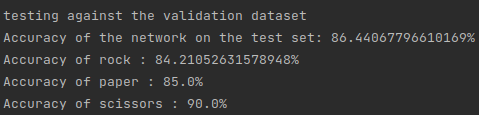
\includegraphics[width=0.8\textwidth]{img/TestAccuracy_final_validation.png}
				\caption{Accuracy on validation dataset}
			\end{figure}   
		\end{itemize}
	\end{frame}

	\begin{frame}{Confusion Matrix - Validation Set}
		\begin{columns}
			\begin{column}{.5\textwidth}
				\begin{figure}
					\centering
					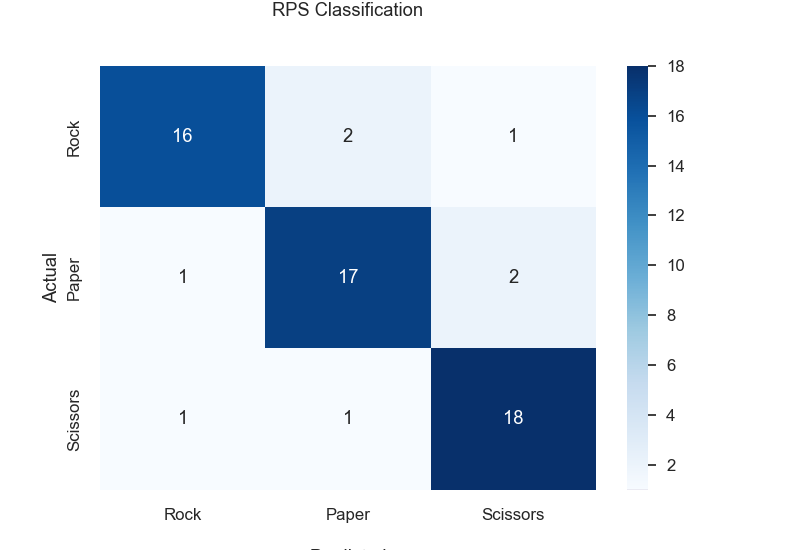
\includegraphics[width=1\textwidth]{img/CFM_final_validation_numeric.png}
					\caption{Numeric CM of testset}
				\end{figure}      
			\end{column}
			\begin{column}{.5\textwidth}
				\begin{figure}
					\centering
					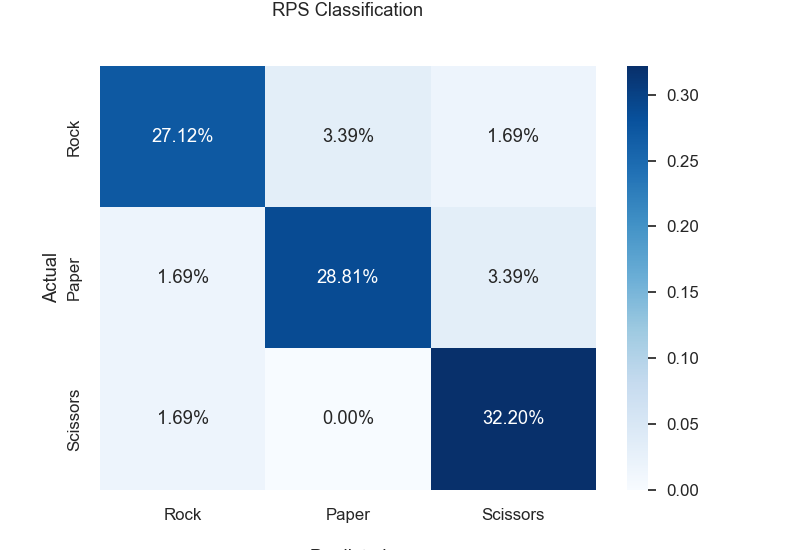
\includegraphics[width=1\textwidth]{img/CFM_final_validation_percent.png}
					\caption{CM of testset (in \%)}
				\end{figure}      
			\end{column} 
		\end{columns}
	\end{frame}
	
	\begin{frame}{Model Performance - Test Data}
	How well did our model perform on the provided test data?
	\begin{itemize}
		\item more custom made data
		\item no images of big datasets (significant portion of training data)
		\item unseen
		\pause
		\item model performance:
		\newline
		\begin{figure}
			\centering
			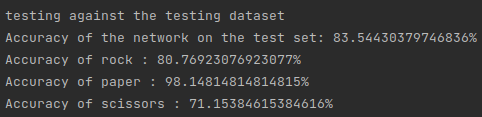
\includegraphics[width=0.8\textwidth]{img/TestAccuracy_final_test.png}
			\caption{accuracy on test dataset}
		\end{figure}   
	\end{itemize}
	\end{frame}

	\begin{frame}{Confusion Matrix - Unseen Testset}
		\begin{columns}
			\begin{column}{.5\textwidth}
				\begin{figure}
					\centering
					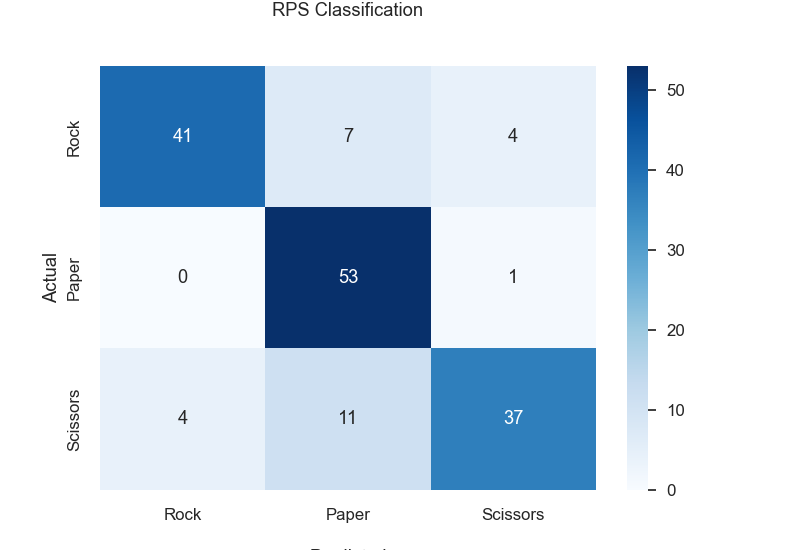
\includegraphics[width=1\textwidth]{img/CFM_final_test_numeric.png}
					\caption{Numeric CM of unseen testset}
				\end{figure}      
			\end{column}
			\begin{column}{.5\textwidth}
				\begin{figure}
					\centering
					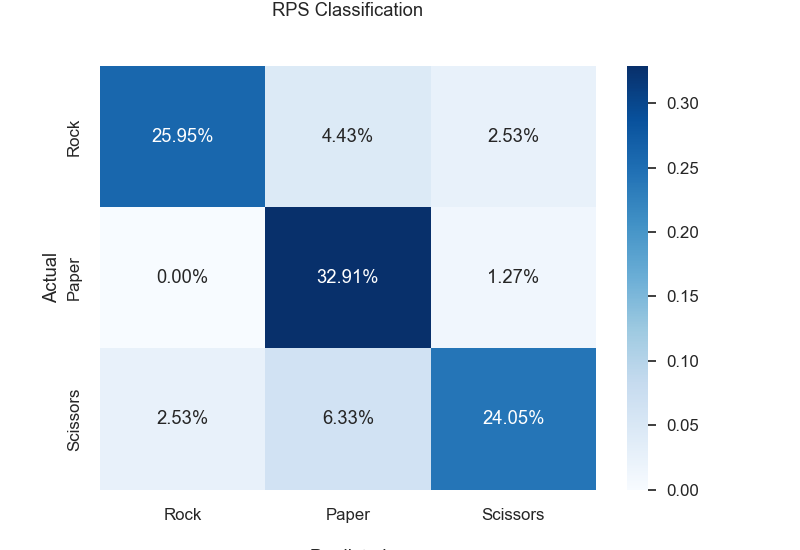
\includegraphics[width=1\textwidth]{img/CFM_final_test_percent.png}
					\caption{CM of unseen testset (in \%)}
				\end{figure}      
			\end{column} 
		\end{columns}
	\end{frame}

\section{Evaluating On Distorted Images}
	\begin{frame}{Image Distortion - Random Distortion}
		Each pixel has a chance to be removed (25\%):
		\begin{figure}
			\centering
			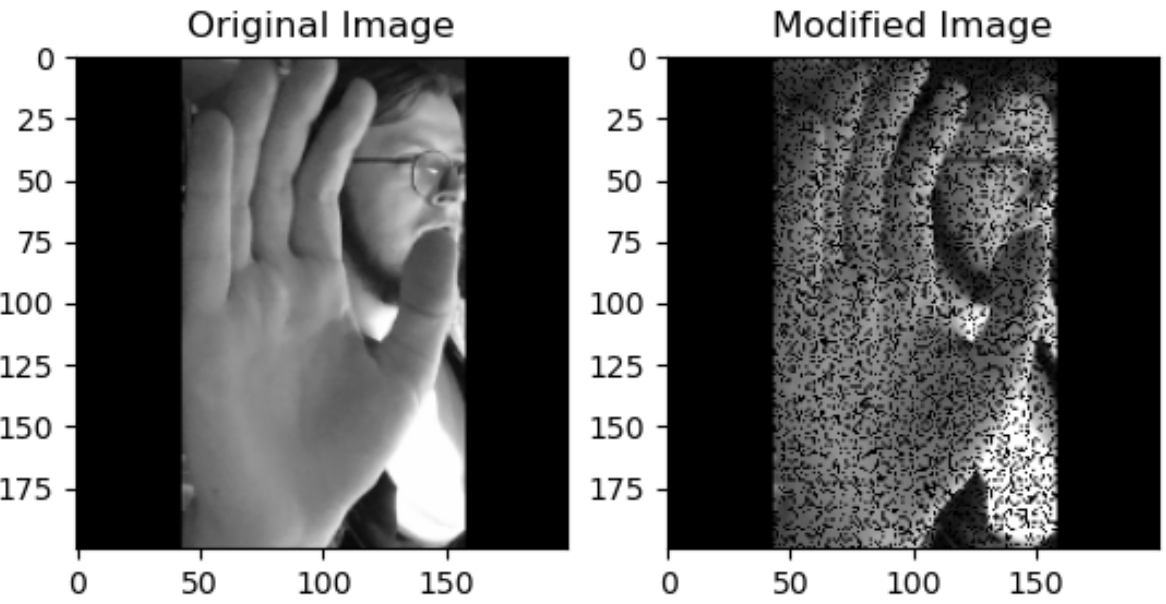
\includegraphics[width=0.7\textwidth]{img/randomDistortion1.png}
			\caption{random distortion with a pixel elimination probability of 25\%}
		\end{figure}
	\end{frame}

	\begin{frame}{Image Distortion - Gaussian Distortion}
	Gaussian Filter:
		\begin{itemize}
			\item follows normal distribution
			\item parameter: standard deviation (25 in our case)
		\end{itemize}
	\pause
		\begin{figure}
			\centering
			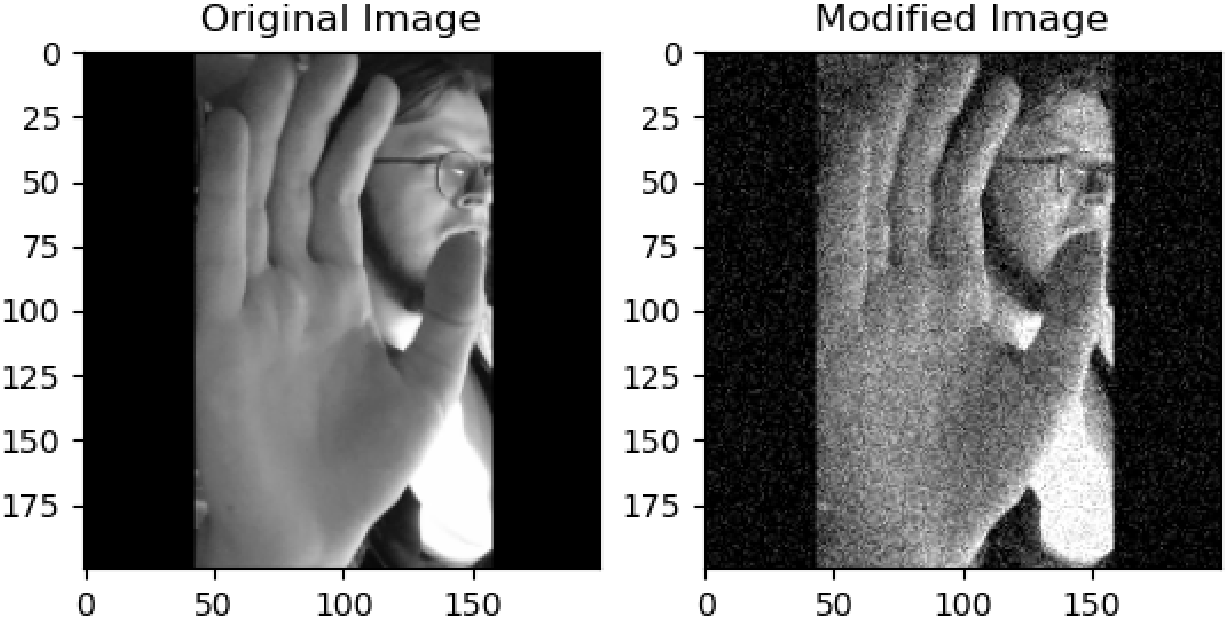
\includegraphics[width=0.55\textwidth]{img/gaussianDistortion1.png}
			\caption{distortion using a Gaussian filter with SD = 25}
		\end{figure}
	\end{frame}
	
	
	\begin{frame}{Model Performance on distorted data}
		Random Distortion:
		\begin{figure}
			\centering
			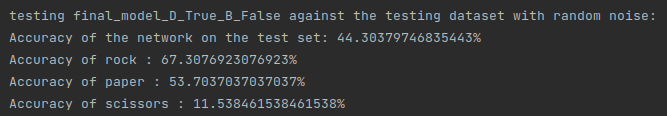
\includegraphics[width=1\textwidth]{img/TestAccuracy_final_test_rm.png}
			\caption{Accuracy on randomly distorted testset}
		\end{figure}   
	\end{frame}

	\begin{frame}
		Gaussian Distortion:
		\begin{figure}
			\centering
			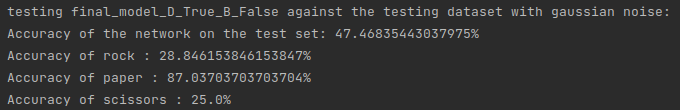
\includegraphics[width=1\textwidth]{img/TestAccuracy_final_test_gauss.png}
			\caption{Accuracy on testset distorted with a Gaussian filter}
		\end{figure}   
	\end{frame}

	\begin{frame}{Random Distortion - Confusion Matrix}
		\begin{columns}
			\begin{column}{.5\textwidth}
				\begin{figure}
					\centering
					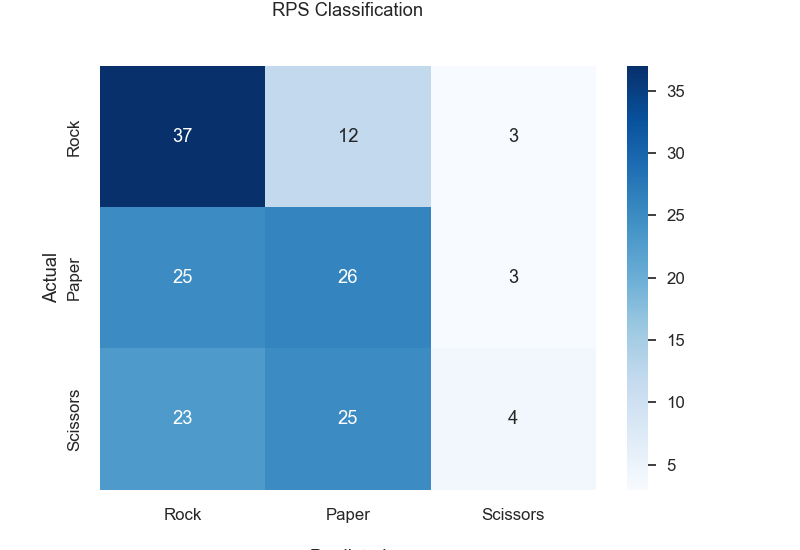
\includegraphics[width=1\textwidth]{img/CFM_final_test_rm_numeric.png}
					\caption{Numeric CM of distorted testset}
				\end{figure}      
			\end{column}
			\begin{column}{.5\textwidth}
				\begin{figure}
					\centering
					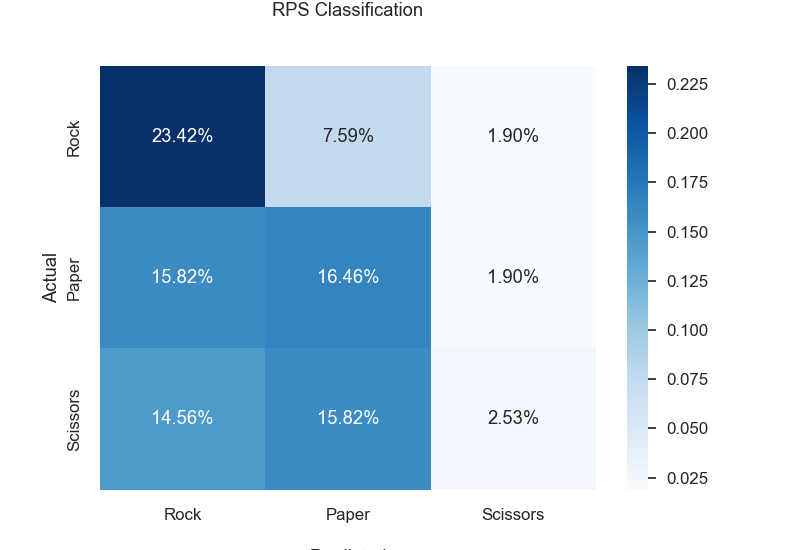
\includegraphics[width=\textwidth]{img/CFM_final_test_rm_percent.png}
					\caption{CM of distorted testset (in \%)}
				\end{figure}      
			\end{column} 
		\end{columns}  
	\end{frame}

	\begin{frame}{Gaussian Distortion - Confusion Matrix}
		\begin{columns}
			\begin{column}{.5\textwidth}
				\begin{figure}
					\centering
					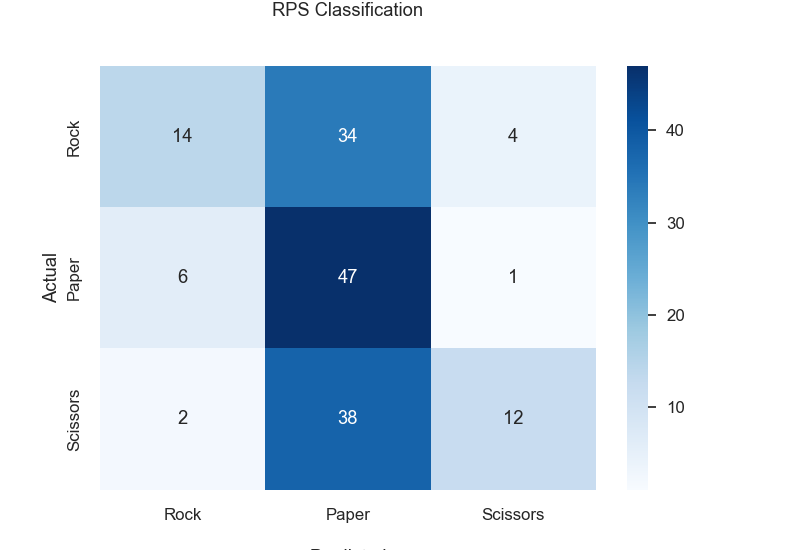
\includegraphics[width=1\textwidth]{img/CFM_final_test_gauss_numeric.png}
					\caption{Numeric CM of distorted testset}
				\end{figure}      
			\end{column}
			\begin{column}{.5\textwidth}
				\begin{figure}
					\centering
					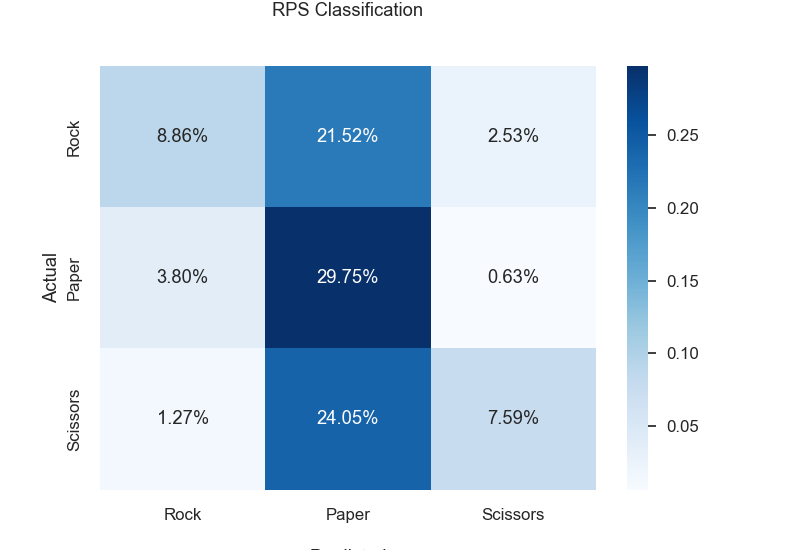
\includegraphics[width=\textwidth]{img/CFM_final_test_gauss_percent.png}
					\caption{CM of distorted testset (in \%)}
				\end{figure}      
			\end{column} 
		\end{columns}  
	\end{frame}

	\begin{frame}{Performances on Different Test Data}
		\begin{table}[]
			\begin{tabular}{@{}lcccc@{}}
				\toprule
				& \textbf{Old} & \multicolumn{1}{l}{\textbf{Current}} & \multicolumn{1}{l}{\textbf{No Regularization}} & \multicolumn{1}{l}{\textbf{With Noisy Data}} \\ \midrule
				\textbf{Undistorted Testset}    & 67.8\%       & 83.5\%                               & 80.4\%                                         & 61.4\%                                       \\
				\textbf{Random Distortion}   & 42.4\%       & 44.3\%                               & 38.0\%                                         & 64.4\%                                       \\
				\textbf{Gaussian Distortion} & 55.9\%       & 47.5\%                               & 58.2\%                                         & 63.3\%                                       \\ \bottomrule
			\end{tabular}
			\caption{Performance comparison of various models on different test data}
			\label{tab:my-table}
		\end{table}
	\end{frame}

	\section{Conclusion}
		\begin{frame}{Conclusion}
		Things we learned evaluating our model:
		\begin{itemize}
			\item better performing model $\neq$ more robust model
			\item big impact of noisy data
			\item robustness can be improved by training with noisy data
		\end{itemize}
		\pause
		Answering our research question: \\
		\pop{The usage of distorted test data does lead to a worse model performance compared to the same test data without distortion.} 
		\end{frame}
}

% finally our last stuff
\appendix
{\nologo
	\begin{frame}[standout]
		Thank you!
	\end{frame}
}
\end{document}